\documentclass{assignment}

\usepackage{graphicx}
\usepackage{listings}

\title{Model Proposal for Large-Scale FPS PVP Game Balance}
\author{Silas Falde}
\class{CMPLXSYS 531 - Computer Modeling of Complex Systems}
\date\today

\begin{document}
\maketitle

\section{Overview}

\paragraph{Goal}

Use an agent-based model of large-scale first-person shooter (FPS) player-versus-player (PVP) games to explore the effects of various game balance changes on player experience and game dynamics. The model will simulate player interactions, weapon usage, and game mechanics to assess how different balance adjustments impact gameplay, player satisfaction, and overall game health. Primary balance factors of interest will include map design, player team assignment, and weapon balance.

\paragraph{Rationale}

An agent-based approach is appropriate because FPS PVP balance emerges from many individual player decisions and interactions rather than from a single aggregate rule. By modeling players as heterogeneous agents acting within a shared environment, the simulation can capture how map layout, team assignment, and weapon statistics influence outcomes such as engagement frequency, fairness, and player satisfaction. This makes it well suited for testing balance changes in a controlled setting before applying them in practice.

\paragraph{Main Processes of Interest}

\begin{itemize}
    \item \textbf{Player-to-Player Engagement:} Individual agents detect and engage nearby enemies, with engagement outcomes (winner/loser) determined by player skill, weapon choice, positioning, etc. At the macro level, this generates kill/death ratios and engagement frequency distributions that indicate overall game competitiveness.

    \item \textbf{Objective-Oriented Movement:} Player agents navigate toward team objectives based on map layout and team strategy. Micro-level pathfinding and positioning decisions aggregate into macro-level team progress rates, objective capture times, and coordination effectiveness.

    \item \textbf{Team Dynamics and Success:} Individual player performance and positioning influence small group cohesion and team-wide success metrics. Emergent team-level dynamics include win rates, spatial clustering around objectives, and overall team K/D ratios that reflect balance across matched teams.

    \item \textbf{Weapon and Utility Selection:} Agent choices regarding weapon loadouts and ability usage create feedback loops affecting engagement outcomes. Aggregate weapon usage patterns and their correlation with team success reveal whether certain weapons or strategies dominate, indicating balance issues.
\end{itemize}

\paragraph{Design Concepts}
\begin{itemize}
    \item \textbf{{Emergence:}} Team-level balance and fairness metrics emerge from individual player decisions about positioning, weapon selection, and engagement timing. No explicit rules enforce balanced outcomes; instead, they arise from heterogeneous agent interactions within the shared game environment.

    \item \textbf{{Adaptation:}} Player agents adapt their behavior based on local information, including enemy positions, available weapons, and team objectives. Agents adjust movement patterns and engagement strategies in response to observed outcomes and environmental constraints.

    \item \textbf{{Objectives:}} Individual agents pursue personal objectives (eliminating enemies, surviving) while contributing to team objectives (capturing points, winning rounds). This hierarchical objective structure generates tension between individual and collective success.

    \item \textbf{{Learning:}} Agents may modify weapon and ability selection based on recent engagement success rates, creating feedback loops that amplify or suppress certain strategies over a simulation run.

    \item \textbf{{Heterogeneity:}} Players are heterogeneous in skill level, weapon preference, and positional awareness. This heterogeneity is essential for capturing realistic team composition effects and their influence on balance.

    \item \textbf{{Stochasticity:}} Engagement outcomes incorporate stochastic elements representing uncertainty in player aim, ability activation, and environmental factors. This prevents deterministic behavior and generates varied gameplay outcomes from identical initial conditions.
\end{itemize}

\section{Model}

This agent-based model simulates FPS PVP matches using discrete-time steps where player agents navigate a grid-based map, engage in stochastic combat, and adapt weapon/positioning decisions. Agents are heterogeneous players with varying skill levels that interact within a shared environment through line-of-sight detection and combat resolution, with time advancing in fixed intervals representing game ticks. Figure \ref{fig:model-diagram} illustrates the overall structure of the model, while Figure \ref{fig:timestep-flowchart} details the sequence of operations performed at each time step.

\begin{figure}
    \centering
    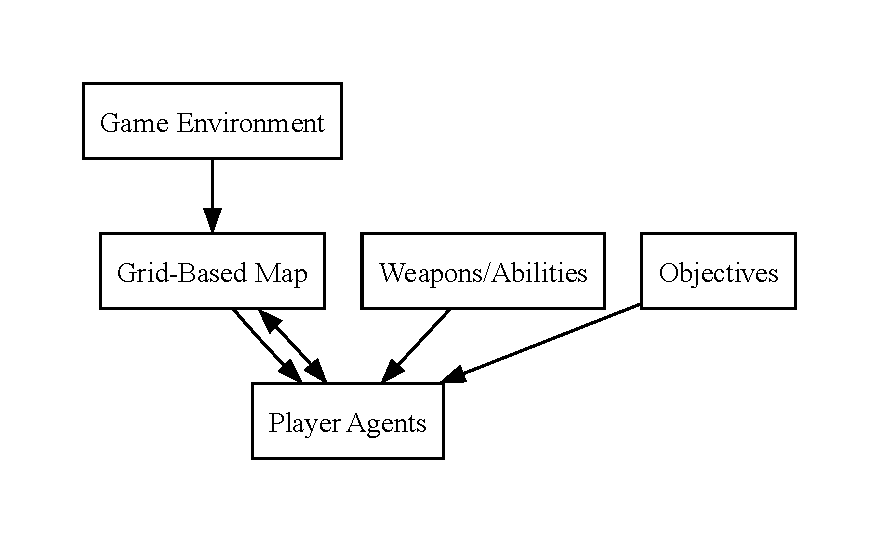
\includegraphics[scale=0.5]{model-diagram.pdf}
    \caption{Schematic of the agent-based model structure, showing player agents interacting within a shared environment, making decisions based on local information, and generating emergent team-level dynamics.}
    \label{fig:model-diagram}
\end{figure}

\begin{figure}
    \centering
    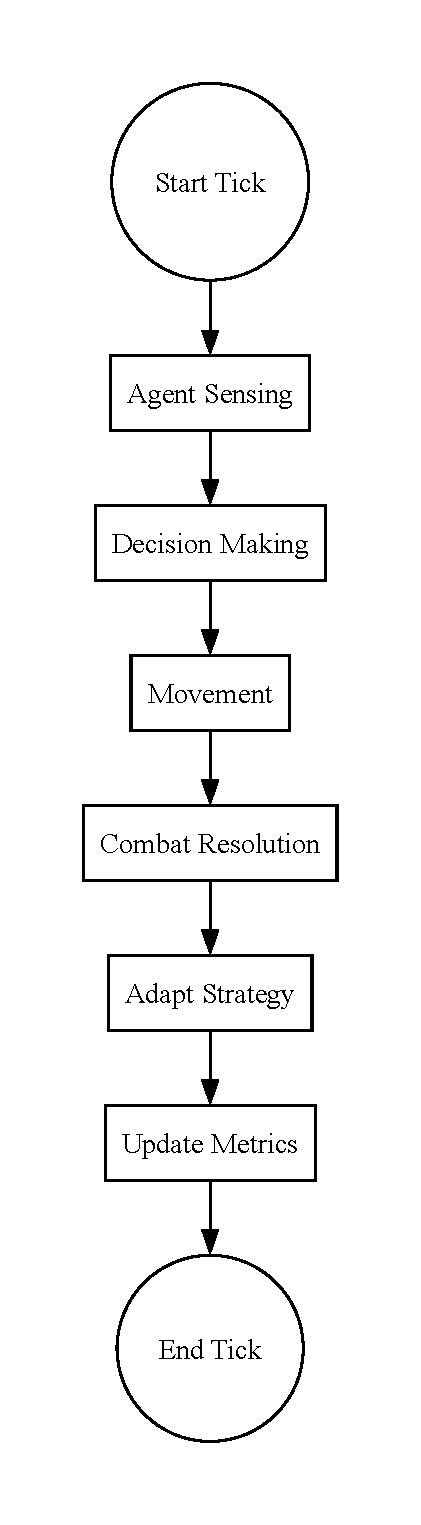
\includegraphics[scale=0.5]{timestep-flowchart.pdf}
    \caption{Flowchart of the timestep structure, illustrating the sequence of operations performed at each discrete time step.}
    \label{fig:timestep-flowchart}
\end{figure}

\paragraph{Environment}
The environment is a finite, two-dimensional grid representing an FPS map. Each cell corresponds to a traversable space or an obstacle and stores static map attributes (cover level, sight blocking, and objective membership) plus dynamic state variables that change over time (current occupants, contested status, and recent combat intensity). Boundary conditions are non-wrapping: agents cannot move beyond map edges, and edge cells behave as hard boundaries. This keeps geometry faithful to arena-style shooter maps rather than toroidal worlds.

Environment structure and properties are defined as follows. (1) \textbf{Dimensionality and topology:} a discrete 2D lattice with Moore or von Neumann local neighborhoods (implementation choice), where movement and detection are constrained by adjacency and line-of-sight. (2) \textbf{Terrain classes:} cells are tagged as open lane, cover, choke point, spawn zone, or objective zone; these tags influence movement cost, visibility, and engagement probability. (3) \textbf{Objective fields:} objective cells maintain capture progress and controlling team, creating local incentives that pull agent movement and concentrate conflict. (4) \textbf{Visibility field:} line-of-sight is computed from obstacle layout and used by sensing and targeting procedures.

The environment is mostly static in geometry during a match (walls and map layout do not change), but it evolves through procedural updates each tick. At every time step, the model updates objective control state, occupancy maps, local pressure/heat maps from recent combat, and spawn availability after eliminations. These environment-level processes feed back into agent behavior by altering path desirability, exposure risk, and engagement opportunities. In turn, aggregated agent actions (movement, clustering, combat outcomes) modify the environment's dynamic fields, producing coupled agent-environment feedback over the simulation horizon.

\paragraph{Agents}
Agents represent individual players with persistent state including unique ID, team, location, health/alive status, weapon loadout, skill parameters (e.g., accuracy and aggression), and short-term performance memory. At each tick, an agent senses local enemies/objectives, chooses a movement or engagement action, may attack if an opponent is visible and in range, contributes to capture/defense when in objective zones, and respawns after elimination; these actions alter the agent's own state (health, ammo, cooldowns, position), other agents' states (damage/elimination), and environment fields (occupancy, objective control, and local combat intensity). Action selection follows conditional rules based on agent properties and context: dead agents wait to respawn, alive agents engage when an engagement score exceeds a threshold, otherwise they reposition toward objectives or cover according to risk/objective preferences, and then update strategy weights from recent outcomes. Interaction topology is spatial rather than perfectly mixed: agents interact primarily with nearby or line-of-sight agents on the 2D grid, while also interacting with the environment by reading terrain/objective information and writing back dynamic map state through movement and combat.

\paragraph{Scheduling}

Each match is simulated in discrete ticks, and each tick follows the same ordered pipeline (Figure \ref{fig:timestep-flowchart}):
\begin{enumerate}
    \item \textbf{Sense:} Every alive agent reads local observations (visible enemies, teammate proximity, nearby cover, and objective status), while dead agents only update respawn timers.
    \item \textbf{Decide:} Each alive agent computes an action choice (engage, reposition, push objective, hold/defend, or retreat) from its internal state and local context.
    \item \textbf{Move:} Movement actions are applied to update agent positions on the grid, respecting obstacles, boundaries, and occupancy constraints.
    \item \textbf{Resolve Combat:} Attacks for agents with valid targets are resolved stochastically, updating health, eliminations, ammo/cooldowns, and kill/death events.
    \item \textbf{Update Objectives and Environment:} Objective capture/contest values are updated from current local presence; occupancy maps, combat heat/pressure fields, and spawn availability are refreshed.
    \item \textbf{Adapt:} Agents update short-term strategy weights (e.g., aggression or weapon preference) from recent outcomes, and respawn eligible agents at valid spawn cells.
    \item \textbf{Record Metrics:} The model logs tick-level outputs (engagement frequency, objective control, team K/D, clustering, and win-condition progress) before advancing to the next tick.
\end{enumerate}
This schedule is synchronous at the tick level (all agents follow the same phase order), with interaction effects emerging from shared environment updates and local spatial conflicts.

\paragraph{Parameters}
Global parameters are fixed at the start of each run (unless intentionally varied during experiments) and include:
\begin{itemize}
    \item \textbf{Map and geometry:} grid width/height, obstacle density/layout, cover distribution, number and location of objective zones, and spawn zone locations.
    \item \textbf{Population and teams:} total number of agents, team sizes, team assignment policy (balanced/random), and initial spawn allocation policy.
    \item \textbf{Combat mechanics:} base weapon damage, weapon ranges, fire-rate/cooldown values, engagement noise/stochasticity level, and line-of-sight radius.
    \item \textbf{Agent heterogeneity distributions:} sampling distributions for skill, reaction delay, aggression, risk tolerance, and objective priority.
    \item \textbf{Objective and scoring rules:} capture rate, contest decay/reset behavior, win-condition thresholds, and match time limit (maximum ticks).
    \item \textbf{Respawn and recovery:} respawn delay, spawn protection (if used), and post-respawn state reset rules.
    \item \textbf{Simulation controls:} random seed, number of replications per parameter setting, metric logging interval, and adaptation/learning rate.
\end{itemize}

Model initialization occurs in a fixed setup sequence before the first tick: (1) choose a global parameter set and random seed; (2) generate/load the map and precompute static fields such as traversability and line-of-sight blockers; (3) create agents with unique IDs and sample their heterogeneous traits from the specified distributions; (4) assign teams and initial loadouts; (5) place agents in valid spawn cells while enforcing occupancy constraints; (6) initialize objective state (neutral or pre-owned, depending on scenario), occupancy maps, and heat/pressure maps to baseline values; and (7) reset all counters/metrics (kills, deaths, objective progress, team scores) and start the simulation clock at tick $t=0$.

Alternatively, parameters could be initialized using real-world Battlefield V stats using the repository found at \url{https://github.com/chastertlye/battlefield-stats-scraper}, which contains data on weapon usage, player performance, and map statistics. This would allow the model to be grounded in empirical data and provide a more realistic baseline for testing balance changes.

\paragraph{Assessment}
Model outcomes will be assessed using both quantitative metrics and qualitative pattern checks. Quantitative metrics include: (1) \textbf{fairness/competitiveness} (team win-rate gap across repeated matches, score differential distribution, and comeback frequency); (2) \textbf{engagement dynamics} (engagements per tick, mean time-to-first-engagement, mean time-to-kill, and fight duration); (3) \textbf{player-level performance dispersion} (K/D distribution by team, variance in individual contribution, and survival-time distribution); (4) \textbf{objective play} (capture rate, contest time, objective control share by team, and time spent in objective zones); (5) \textbf{spatial behavior} (heat-map entropy, clustering around choke points, lane usage balance, and spawn-camp incidence); and (6) \textbf{strategy diversity and balance health} (weapon pick-rate concentration, win contribution by weapon, and adaptation stability over time). In addition, qualitative features will be checked from trajectory and heat-map visualizations, including whether matches show persistent one-sided snowballing, repetitive dominant strategies, or healthy alternation between attack/defense phases. A balanced configuration is expected to show small average win-rate gaps, moderate engagement tempo, low extreme dominance in weapon picks, and robust objective contesting across runs.

Analyses will be organized to directly answer the main goal of evaluating map, team, and weapon balance changes. First, \textbf{baseline calibration} runs will establish reference distributions for all assessment metrics under default parameters. Second, \textbf{one-factor-at-a-time sensitivity analyses} will vary map structure (cover/choke density), team assignment policy, and weapon parameters independently to estimate directional effects and local elasticities. Third, \textbf{factorial experiments} will test interactions among map, team, and weapon settings to identify non-additive effects (for example, whether a weapon imbalance appears only on high-choke maps). Fourth, \textbf{robustness analysis across random seeds and heterogeneous populations} will check whether conclusions persist under stochastic variation. Fifth, \textbf{multi-objective comparison} will rank candidate balance patches using a composite criterion that rewards fairness, strategic diversity, and objective contest intensity while penalizing extreme snowballing. Where appropriate, comparisons will use confidence intervals and effect sizes across replications rather than single-run outcomes. Together, these analyses will identify which balance adjustments most consistently improve player experience proxies and overall game health in the model.

\paragraph{Exploration}
The parameter sweeps of highest interest are those tied directly to map, team, and weapon balance. Planned sweeps include: (1) \textbf{map structure} via cover density (about 10\% to 50\% of traversable cells) and choke-point density (low/medium/high templates); (2) \textbf{team composition and assignment} via team skill-gap scenarios (mean skill difference from 0 to 0.4 on a normalized 0 to 1 skill scale) and assignment policy (random vs. skill-balanced); (3) \textbf{weapon tuning} via base damage multipliers (0.8 to 1.2 of baseline), effective range multipliers (0.8 to 1.2), and cooldown multipliers (0.8 to 1.25); (4) \textbf{objective pacing} via capture-rate multipliers (0.75 to 1.5) and respawn delay (3 to 12 ticks); and (5) \textbf{behavioral adaptation} via learning-rate values (0 to 0.3). Most sweeps will use 5 to 9 evenly spaced values per parameter, followed by focused refinement around transition regions where outcomes shift sharply.

These sweeps help answer the core goal by showing which balance levers reliably improve fairness and player-experience proxies: map sweeps isolate how geometry drives engagement flow and snowballing risk, team sweeps quantify matchmaking sensitivity, weapon sweeps reveal thresholds where a loadout becomes dominant, and objective/respawn sweeps expose pacing regimes that are too slow or too chaotic. Comparing these sweeps with the assessment metrics (win-rate gap, objective contest intensity, engagement tempo, and strategy diversity) identifies robust parameter regions where gameplay remains competitive and varied rather than one-sided or meta-locked.

\section{Questions and Challenges}
One major challenge is managing model complexity: deciding which mechanics are essential for capturing balance dynamics and which can be simplified without losing validity. Additional challenges include (1) calibrating parameter values so simulated outcomes are plausible rather than arbitrary, especially when mapping game-like mechanics to abstract units; (2) separating signal from stochastic noise, since many replications are required to distinguish real balance effects from random variation; (3) handling interaction effects, where map, team assignment, and weapon tuning may combine nonlinearly and make one-factor conclusions misleading; (4) avoiding overfitting to one map or scenario, so findings generalize across layouts and team compositions; and (5) keeping computational cost manageable as the parameter sweep space grows.

Feedback I would especially value: (1) Which mechanics are the highest priority for a first valid version (MVP) of this model? (2) Are the proposed parameter ranges and metrics sufficient to identify practical balance issues, or are key variables missing? (3) What is a reasonable standard for claiming a change is "meaningfully better" (effect-size threshold, confidence interval criterion, or rank-based criterion)? (4) Should I prioritize broader but shallower sweeps, or narrower but deeper sweeps with more replications? (5) Are there recommended approaches for validating this model against real FPS behavior when only partial empirical data are available?

\section{Code}

My repository for this project is located at \url{https://github.com/silasfalde/fps-pvp-dynamics}, and the main model code is in \texttt{src/fps\_pvp\_abm/model.py}, but it's provided here for reference.

\lstset{
    language=Python,
    basicstyle=\ttfamily\small,
    breaklines=true,
    frame=single,
    numbers=left,
    numberstyle=\tiny,
    showstringspaces=false
}
\lstinputlisting[caption={\texttt{model.py}}]{model.py}

\end{document}